\documentclass[11pt, a4]{article}
\usepackage{listings}
\usepackage{amssymb}
\usepackage{enumitem}
\usepackage{amsmath}
%\usepackage{tfrupee}
\usepackage{pgfplots}
\usepackage{tikz}
\usepackage{enumitem}
\usepackage{multirow}
%\usepackage{fancyhdr}
%\usepackage{lastpage}
\usepackage[export]{adjustbox}
\usepackage{wrapfig}
\usepackage[english]{babel}
\usepackage{amsthm}
\usepackage{multirow}
\usepackage{wrapfig,lipsum,booktabs}
\usepackage{graphicx}
\usepackage{caption}
\usepackage{subcaption}
\usepackage{hyperref}
\usepackage{xcolor}


%\newtheorem{theorem}{Theorem}[section]
%\newtheorem{lemma}[theorem]{Lemma}


%\topmargin -0.1in
% \textheight 11in
%\oddsidemargin -.01in
%\evensidemargin .0in
%\textwidth 6.5in
\definecolor{codegreen}{rgb}{0,0.6,0}
\definecolor{codegray}{rgb}{0.5,0.5,0.5}
\definecolor{codepurple}{rgb}{0.58,0,0.82}
\definecolor{backcolour}{rgb}{0.95,0.95,0.92}

\lstdefinestyle{mystyle}{
	backgroundcolor=\color{backcolour},   
	commentstyle=\color{codegreen},
	keywordstyle=\color{magenta},
	numberstyle=\tiny\color{codegray},
	stringstyle=\color{codepurple},
	basicstyle=\ttfamily\footnotesize,
	breakatwhitespace=false,         
	breaklines=true,                 
	captionpos=b,                    
	keepspaces=true,                 
	numbers=left,                    
	numbersep=5pt,                  
	showspaces=false,                
	showstringspaces=false,
	showtabs=false,                  
	tabsize=2
}

\lstset{style=mystyle}
\begin{document}

	\author{Ritabrata Mandal\\ EE24E009}
	\title{DA6400 : Reinforcement Learning\\ Programming Assignment \#1\\ Report}
	\maketitle
	\medskip
	\newpage
	\tableofcontents
	\newpage
	\section{Introduction}
		\subsection{Environments}
		In this programming task, we are utilize the following \href{https://gymnasium.farama.org/}{\textcolor{magenta}{Gymnasium environments}} for training
		and evaluating your policies. The links associated with the environments contain descriptions
		of each environment.
		\begin{itemize}
			\item \href{https://gymnasium.farama.org/environments/classic_control/cart_pole/}{\textcolor{magenta}{CartPole-v1}} : A pole is attached by an un-actuated joint to a cart, which moves along	a frictionless track. The pendulum is placed upright on the cart and the goal is to
			balance the pole by applying forces in the left and right direction on the cart.
			\item \href{https://gymnasium.farama.org/environments/classic_control/mountain_car/}{\textcolor{magenta}{MountainCar-v0}} : The Mountain Car MDP is a deterministic MDP that consists of a
			car placed stochastically at the bottom of a sinusoidal valley, with the only possible
			actions being the accelerations that can be applied to the car in either direction. The
			goal of the MDP is to strategically accelerate the car to reach the goal state on top of
			the right hill. There are two versions of the mountain car domain in gymnasium: one
			with \textit{discrete actions} and one with \textit{continuous}. This version is the one with discrete
			actions.
			\item \href{https://minigrid.farama.org/environments/minigrid/DynamicObstaclesEnv/}{\textcolor{magenta}{MiniGrid-Dynamic-Obstacles-5x5-v0}} : This environment is an empty
			room with moving obstacles. The goal of the agent is to reach the green goal square
			without colliding with any obstacle. A large penalty is subtracted if the agent collides
			with an obstacle and the episode finishes. This environment is useful to test Dynamic
			Obstacle Avoidance for mobile robots with Reinforcement Learning in Partial Observability.
		\end{itemize}
		\subsection{Algorithms}
		Training each of the below algorithms and assessing their comparative performance.
		\begin{itemize}
			\item \textbf{SARSA}$\rightarrow$ with $\epsilon$-\textbf{greedy exploration}
			\item \textbf{Q-Learning}$\rightarrow$ with \textbf{Softmax exploration}
		\end{itemize}
	\section{Implementation}
		\subsection{\href{https://github.com/RitabrataMandal/RL-DA6400-assignment_1/tree/main/cartpole-v1}{\textcolor{magenta}{CartPole-v1}}}
			\subsubsection{Code Snippets}
%				\lstinputlisting[language=Python, caption=SARSA - Agent]{../cartpole-v1/sarsa_agent.py}
			\subsubsection{SARSA Hyper-Parameter Tuning}  
			Using Weights \& Biases (wandb) with a sweep method based on Bayesian optimization, we identified the best-performing hyper-parameters. Specifically, we set $\alpha \in [0.1, 0.5]$ and $\epsilon \in [0.01, 0.15]$, and ran 2000 episodes while minimizing the regret, defined as \(195 -\) (all-time average return). See the wandb report on this environment \href{https://api.wandb.ai/links/ee24e009-iitm/0hseqrps}{here}. Additionally, Figure \ref{fig:sarsacartpole} displays the results from 50 sweeps, illustrating the relationship between $\alpha$, $\epsilon$, and the reward.
				\begin{figure}[h]
					\centering
					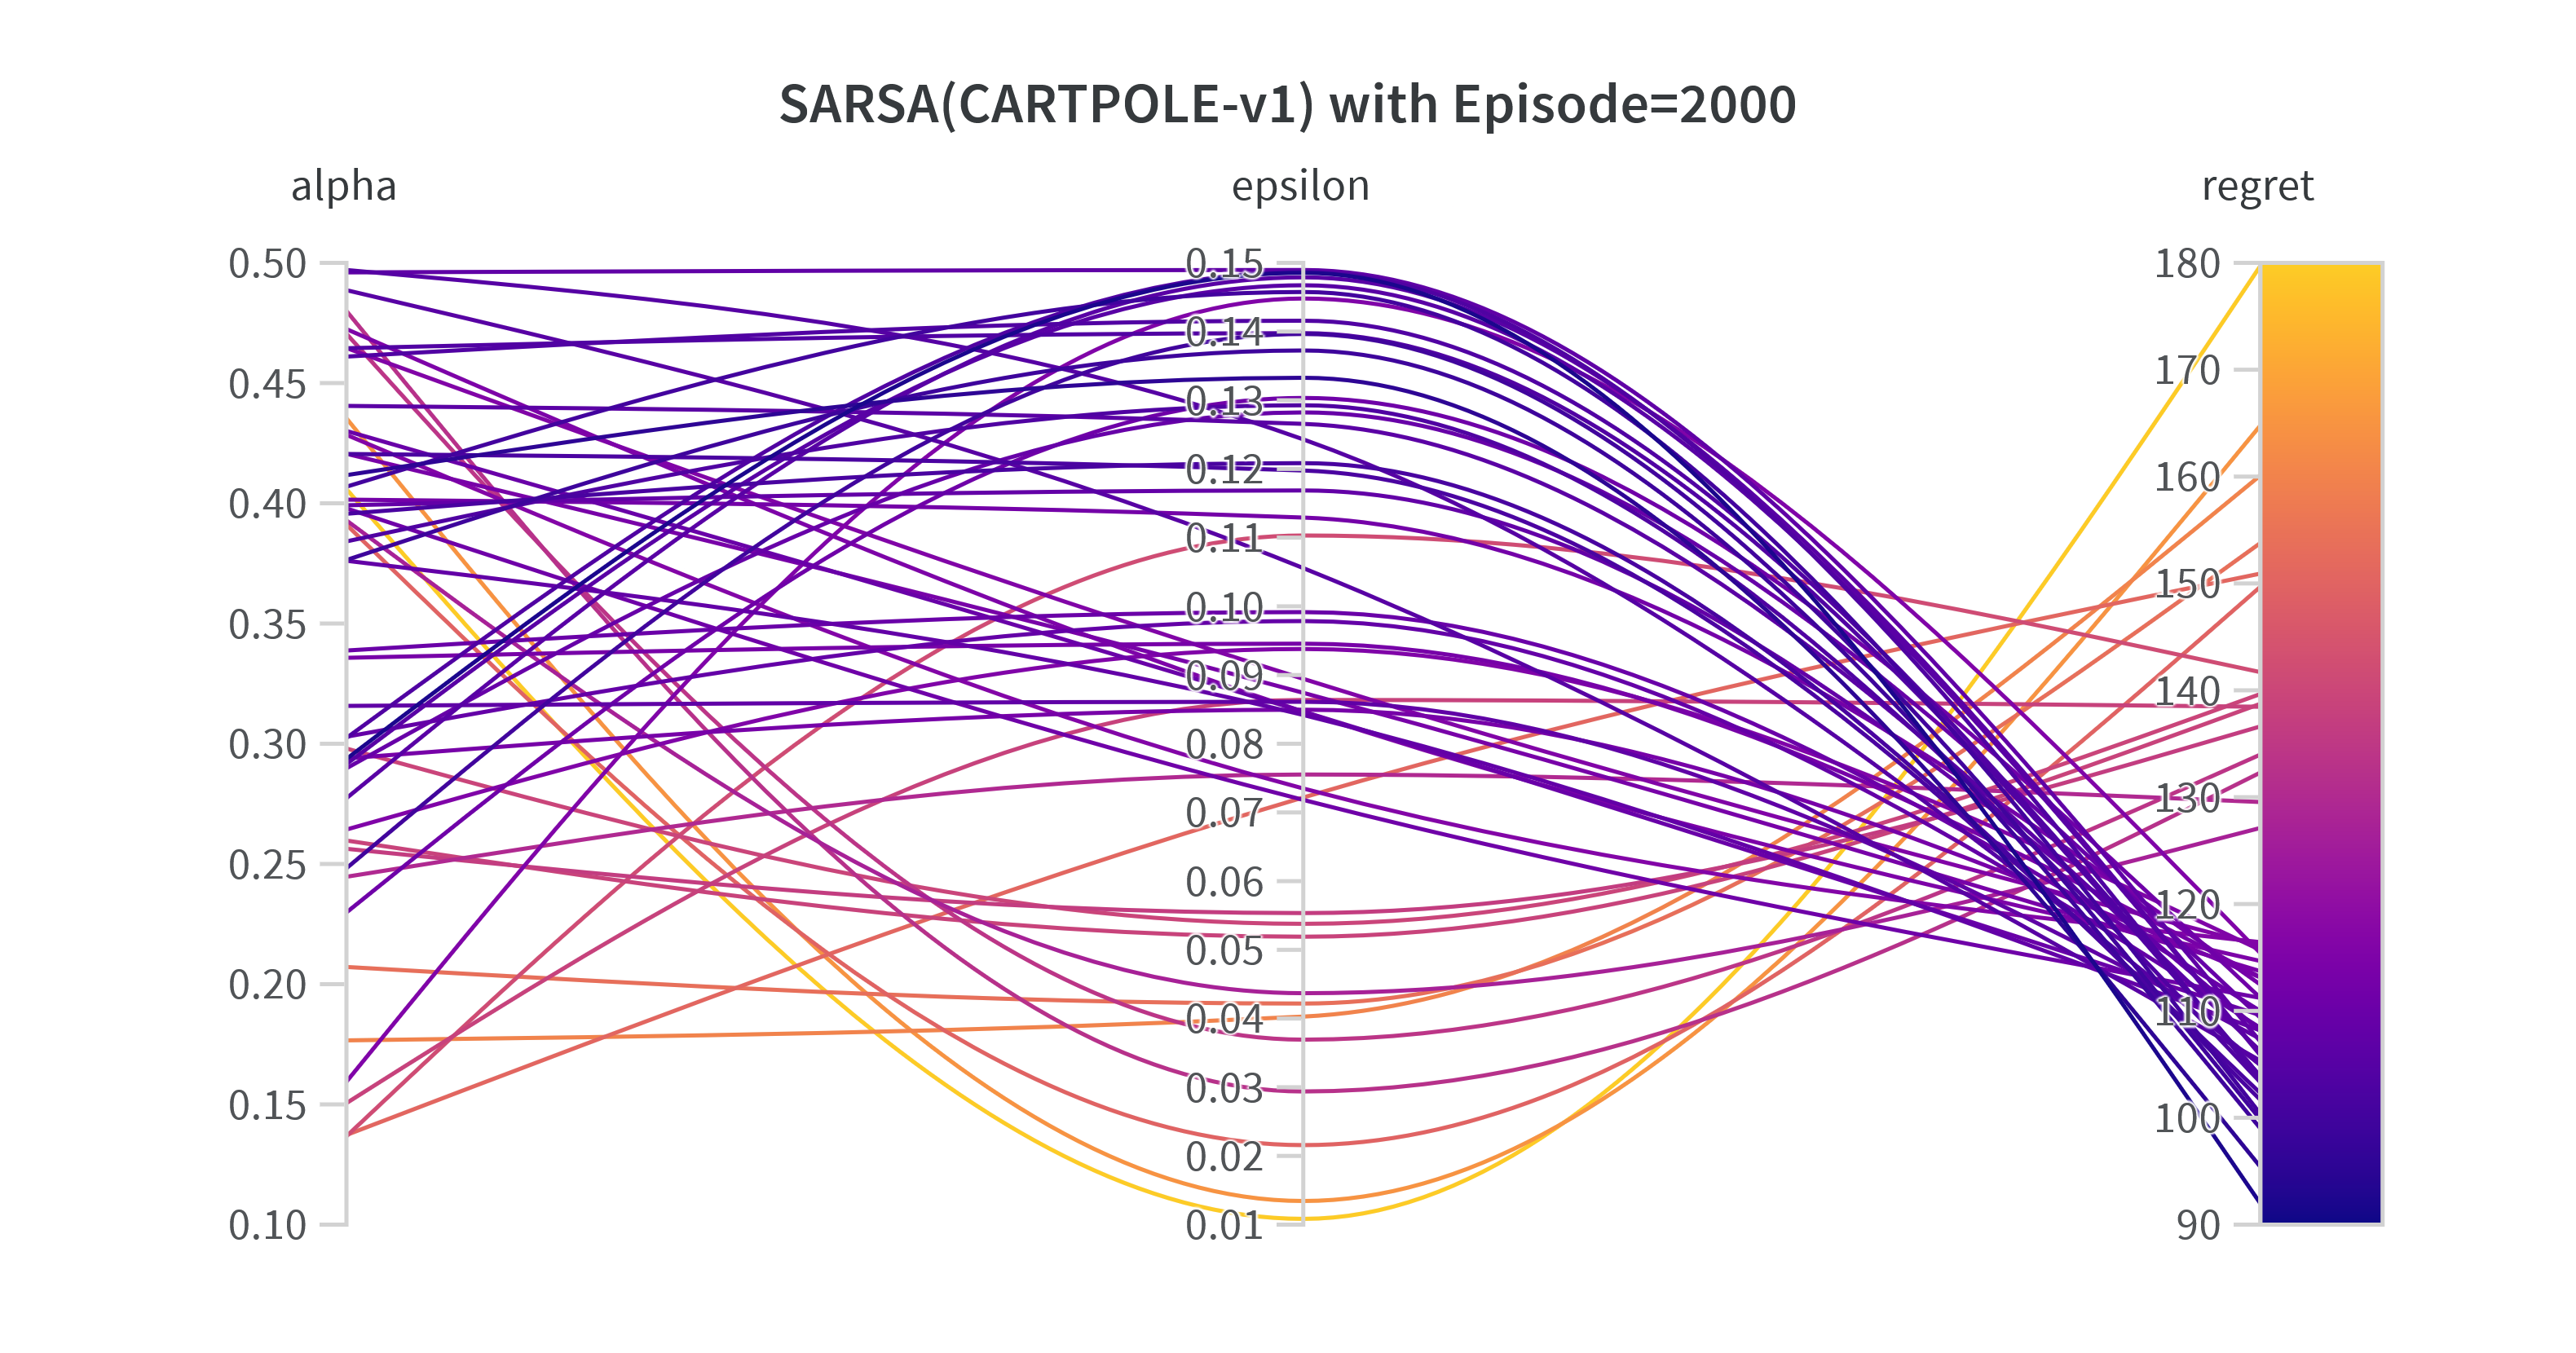
\includegraphics[width=1\linewidth]{sarsa-hyp-tuning-cartpole.png}
					\caption{SARSA hyper-parameter sweeps for $\alpha$ and $\epsilon$ in CartPole-v1(2000 episodes), with lines color-coded by regret.}
					\label{fig:sarsacartpole}
				\end{figure}
			%			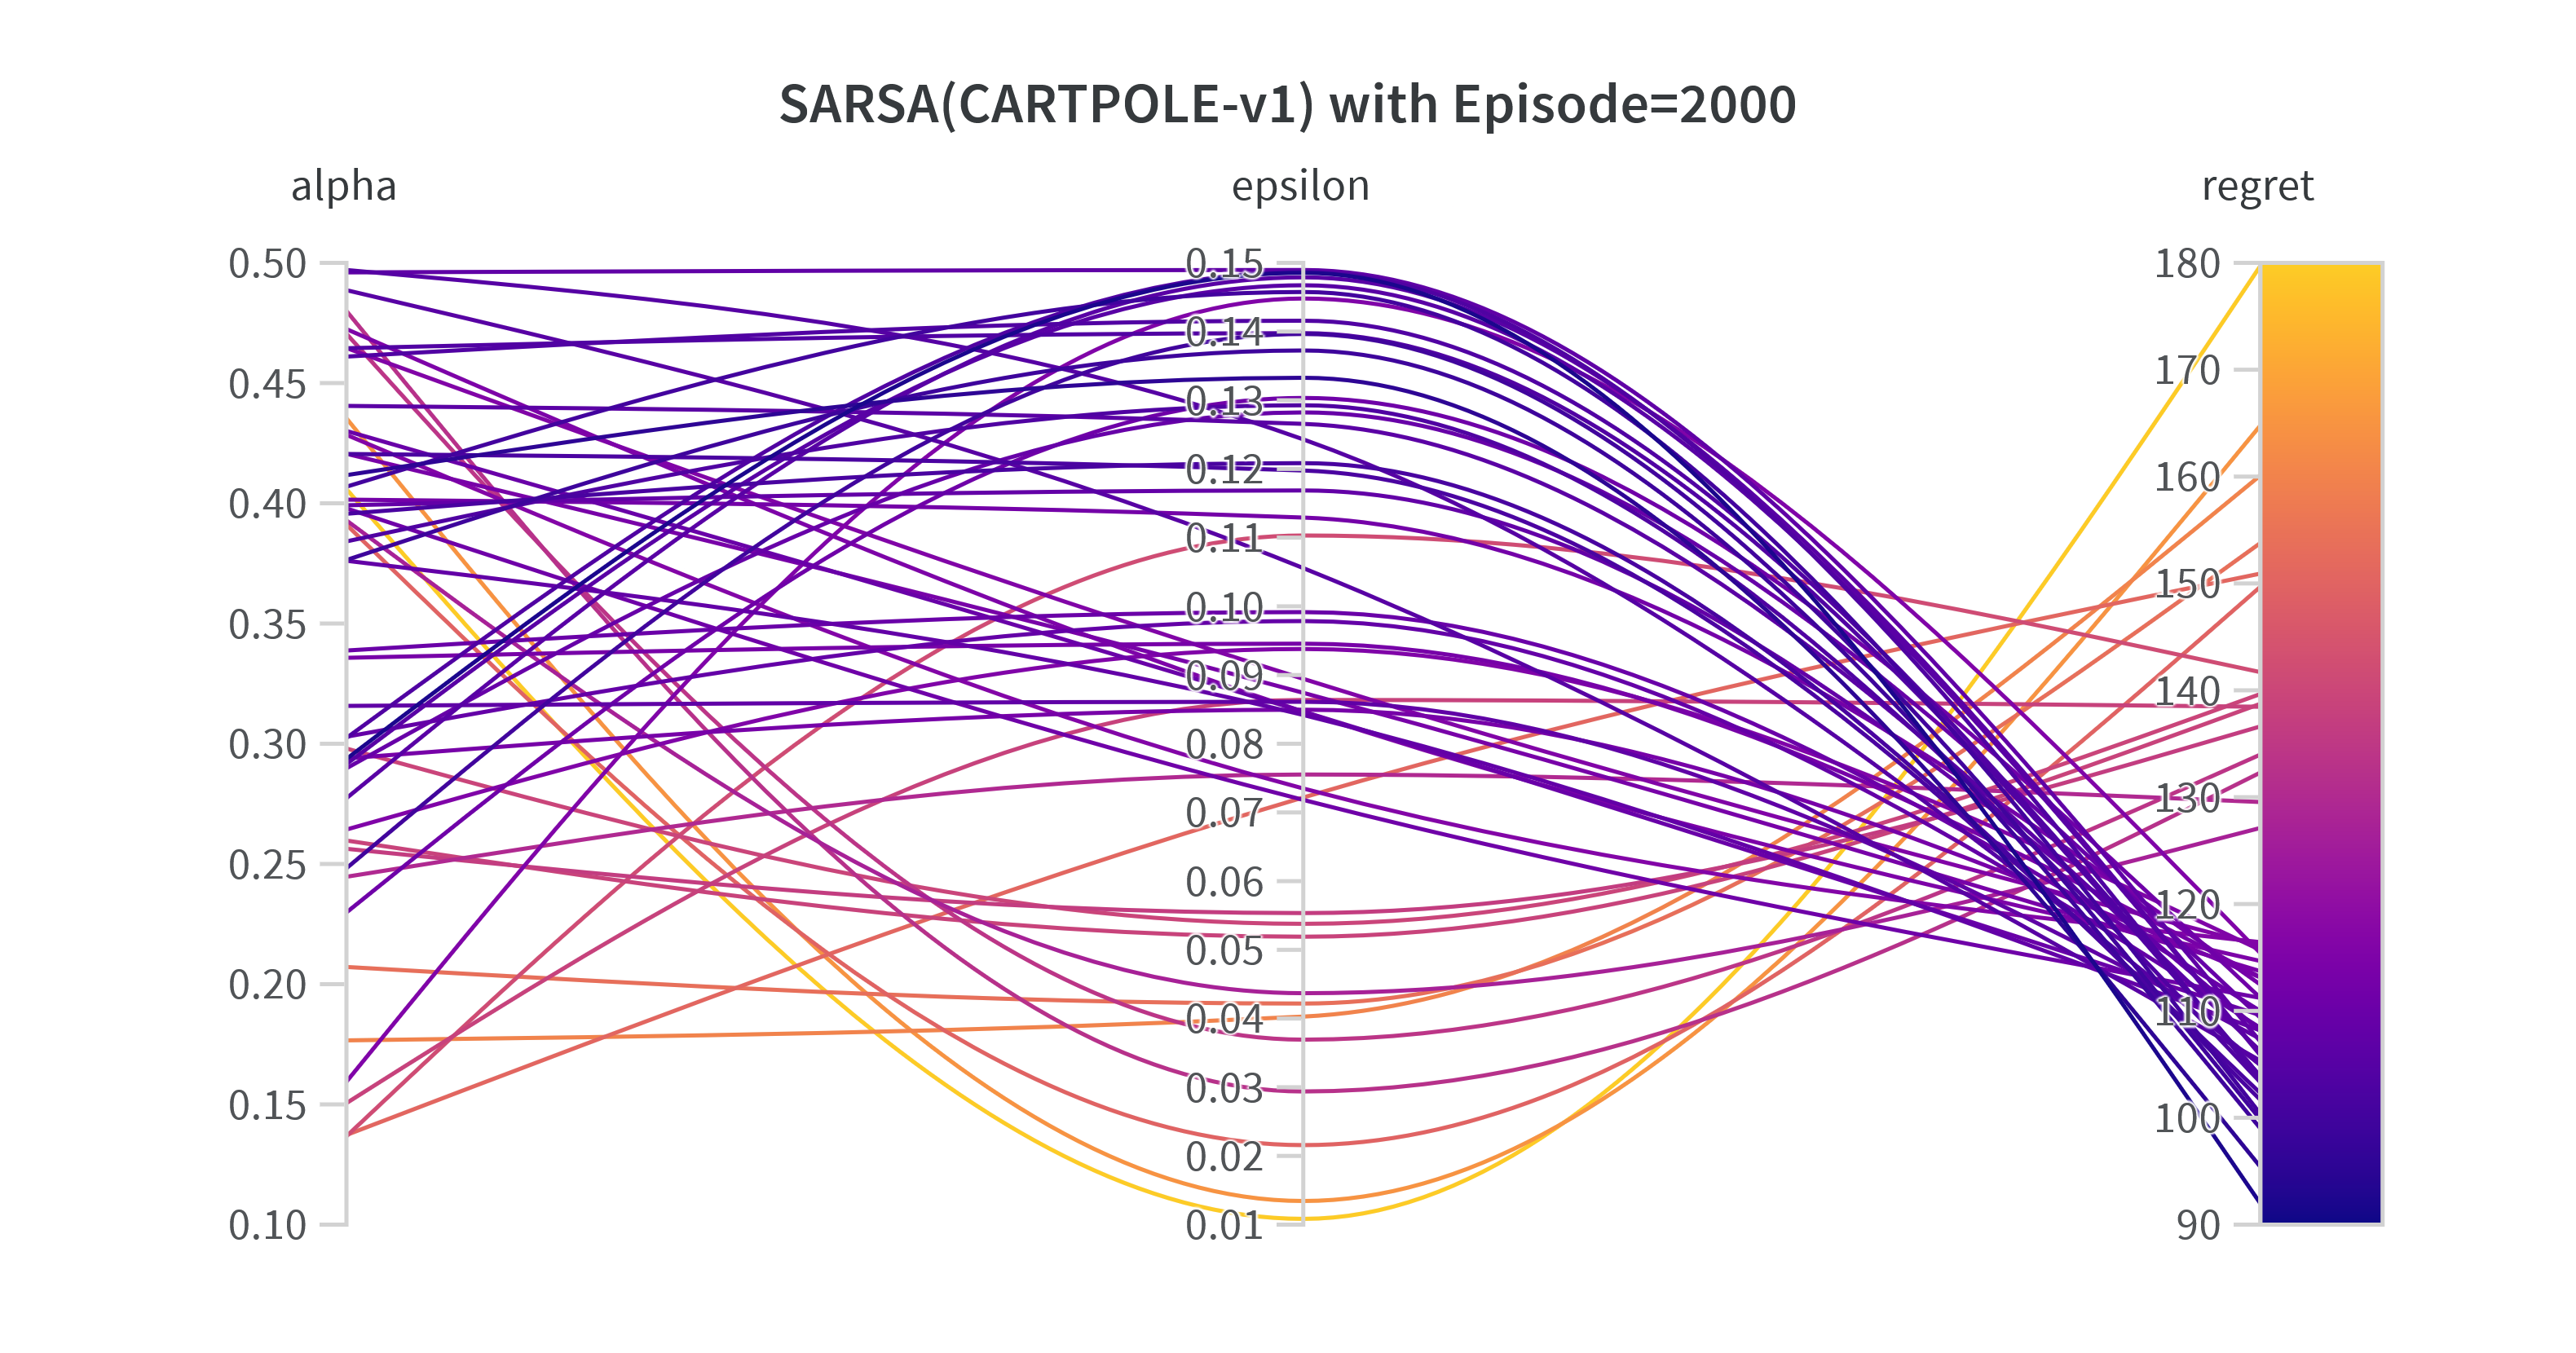
\includegraphics[width=1\linewidth]{sarsa-hyp-tuning-cartpole.png}
			\subsubsection{SARSA best $3$ results}
				\begin{center}
					\begin{tabular}{|c|c|c|c|}
						\hline
						& $\alpha$ & $\epsilon$ & regret\\
						\hline
						1 & 0.29365  & 0.14854 & 91.977\\
						\hline
						2 & 0.4117 & 0.13327 & 95.411\\
						\hline
						3 & 0.3764 & 0.13724 & 98.9932\\
						\hline
					\end{tabular}
				\end{center}
			\subsubsection{Q-Learning hyper-parameter tuning}
			\subsubsection{Q-Learning best $3$ results}
				\begin{center}
					\begin{tabular}{|c|c|c|c|}
						\hline
						& $\alpha$ & $\tau$ & regret\\
						\hline
						1 &  & &\\
						\hline
						2 & & &\\
						\hline
						3 & & &\\
						\hline
					\end{tabular}
					
				\end{center}
			\subsubsection{Result(SARSA vs Q-Learning)}
		\subsection{\href{https://github.com/RitabrataMandal/RL-DA6400-assignment_1/tree/main/mountain_car-v0}{\textcolor{magenta}{MountainCar-v0}}}
			\subsubsection{Code Snippets}
				\lstinputlisting[language=Python,firstline=22, lastline=30, caption=Discretized sates ]{../mountain_car-v0/sarsa.py}
				\lstinputlisting[language=Python,firstline=32, lastline=38, caption=epsilon-greedy action selection]{../mountain_car-v0/sarsa.py}
				\lstinputlisting[language=Python,firstline=41, lastline=79, caption= SARSA implementation ]{../mountain_car-v0/sarsa.py}
				\lstinputlisting[language=Python,firstline=31, lastline=41, caption=Softmax action selection ]{../mountain_car-v0/q_learning.py}
				\lstinputlisting[language=Python,firstline=46, lastline=81, caption=Q-Learning implementation]{../mountain_car-v0/q_learning.py}
			\subsubsection{SARSA  hyper-parameter tuning}
				using wandb with sweep method bayes found the best performing hyper-parameter 
%				\begin{figure}[h]
%					\centering
%					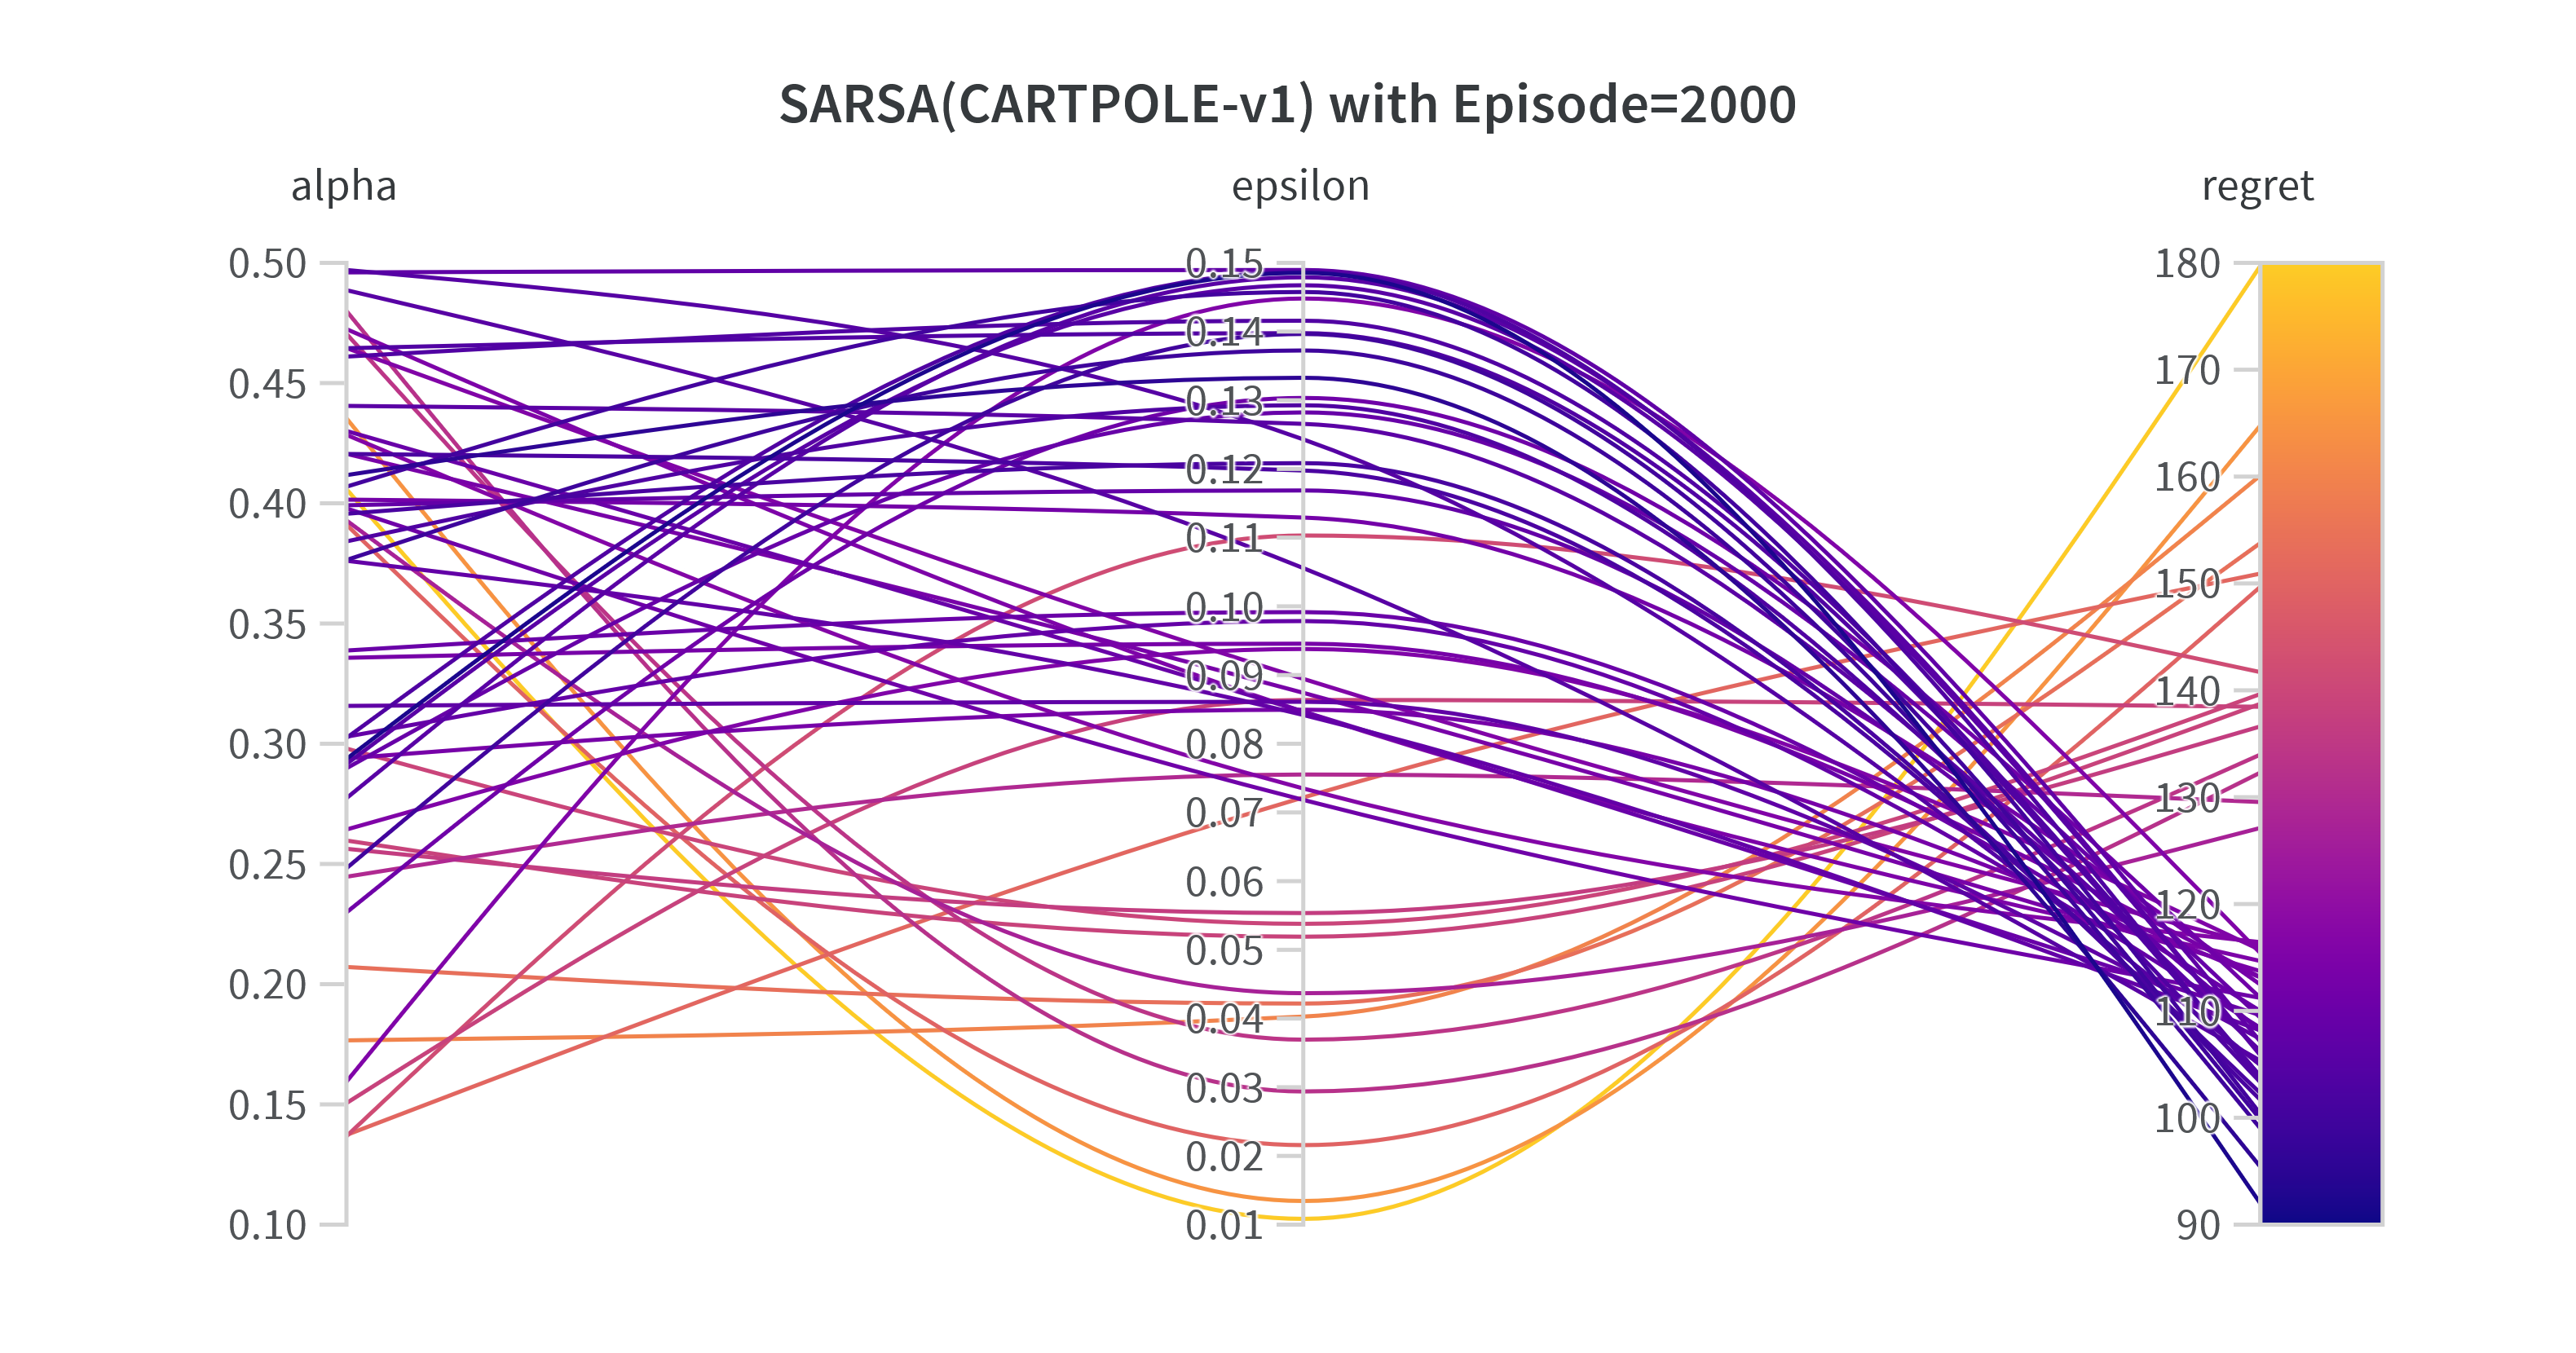
\includegraphics[width=1\linewidth]{sarsa-hyp-tuning-cartpole.png}
%					\caption{}
%					\label{fig:BwR}
%				\end{figure}
			\subsubsection{SARSA best $3$ results}
				\begin{center}
					\begin{tabular}{|c|c|c|c|}
						\hline
						 & $\alpha$ & $\epsilon$ & regret\\
						\hline
						1 & 0.44517 & 0.01104 & 55.5099\\
						\hline
						2 & 0.44469 & 0.010567 & 55.6604 \\
						\hline
						3 & 0.36145 & 0.011928 & 56.547\\
						\hline
					\end{tabular}
				\end{center}

			\subsubsection{Q-Learning hyper-parameter tuning}
			\subsubsection{Q-Learning best $3$ results}
				\begin{center}
					\begin{tabular}{|c|c|c|c|}
						\hline
						& $\alpha$ & $\tau$ & regret\\
						\hline
						1 &  & &\\
						\hline
						2 & & &\\
						\hline
						3 & & &\\
						\hline
					\end{tabular}
				\end{center}
			\subsubsection{Result(SARSA vs Q-Learning)}
		\subsection{\href{https://github.com/RitabrataMandal/RL-DA6400-assignment_1/tree/main/minigrid_world}{\textcolor{magenta}{MiniGrid-Dynamic-Obstacles-5x5-v0}}}
			\subsubsection{Code Snippets}
				\lstinputlisting[language=Python,firstline=7, lastline=11, caption=epsilon-greedy action selection]{../minigrid_world/sarsa.py}
				\lstinputlisting[language=Python,firstline=20, lastline=57, caption= SARSA implementation ]{../minigrid_world/sarsa.py}
				\lstinputlisting[language=Python,firstline=6, lastline=10, caption=Softmax action selection ]{../minigrid_world/q_learning.py}
				\lstinputlisting[language=Python,firstline=15, lastline=55, caption=Q-Learning implementation]{../minigrid_world/q_learning.py}
			\subsubsection{SARSA hyper-parameter tuning}
			\subsubsection{SARSA best $3$ results}
				\begin{center}
					\begin{tabular}{|c|c|c|c|}
						\hline
						& $\alpha$ & $\epsilon$ & regret\\
						\hline
						1 &  & &\\
						\hline
						2 & & &\\
						\hline
						3 & & &\\
						\hline
					\end{tabular}
				\end{center}
			\subsubsection{Q-Learning hyper-parameter tuning}
			\subsubsection{Q-Learning best $3$ results}
				\begin{center}
					\begin{tabular}{|c|c|c|c|}
						\hline
						& $\alpha$ & $\tau$ & regret\\
						\hline
						1 &  & &\\
						\hline
						2 & & &\\
						\hline
						3 & & &\\
						\hline
					\end{tabular}
				\end{center}
			\subsubsection{Result(SARSA vs Q-Learning)}
	\section{Conclusion}
	\section{Github link}	
		 \href{https://github.com/RitabrataMandal/RL-DA6400-assignment_1}{\text{https://github.com/RitabrataMandal/RL-DA6400-assignment\_1}}

	\section{References}
\end{document}